\subsection{Spherical space}
Playing the video game in spherical space gives the impression that the terrain is wallpapered onto the inside of a giant sphere.
Unlike the hyperbolic space, the spherical space is finite.
Comparison in \autoref{fig:spherical-space-games} shows that our implementation provides visual effects to a certain degree similar to those in \textit{Hyperbolica}.
\begin{figure*}[h]
    \centering
    \begin{subfigure}[b]{0.475\textwidth}
        \centering
        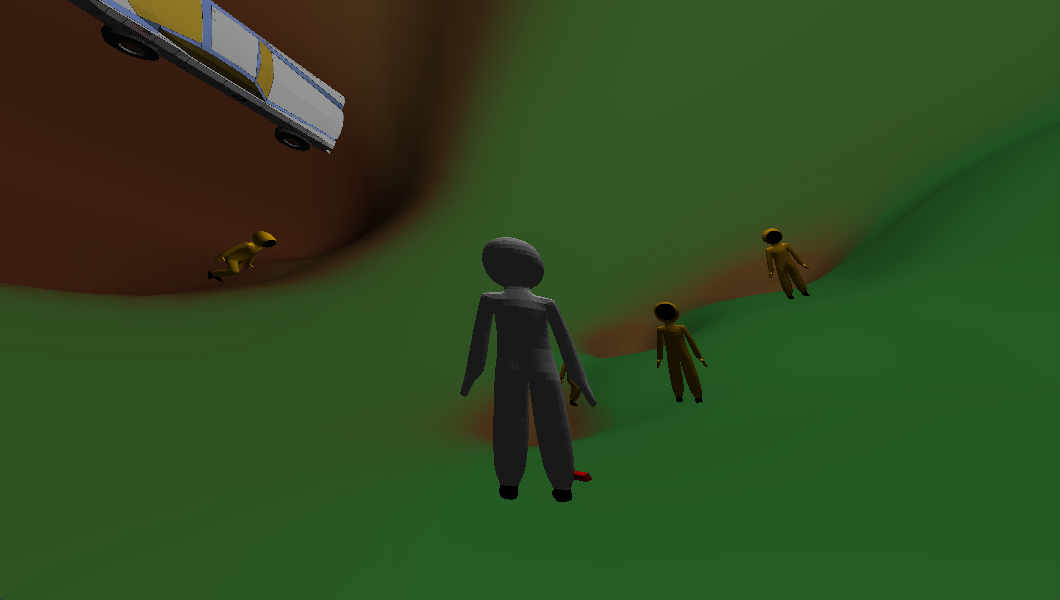
\includegraphics[width=\textwidth]{chapters/results/sections/non_euclidean/resources/spherical-in-hyper.png}
        \caption[]%
        {{\small \textit{Hyper}}}
        \label{fig:spherical-space-games-hyper}
    \end{subfigure}
    \hfill
    \begin{subfigure}[b]{0.5\textwidth}
        \centering
        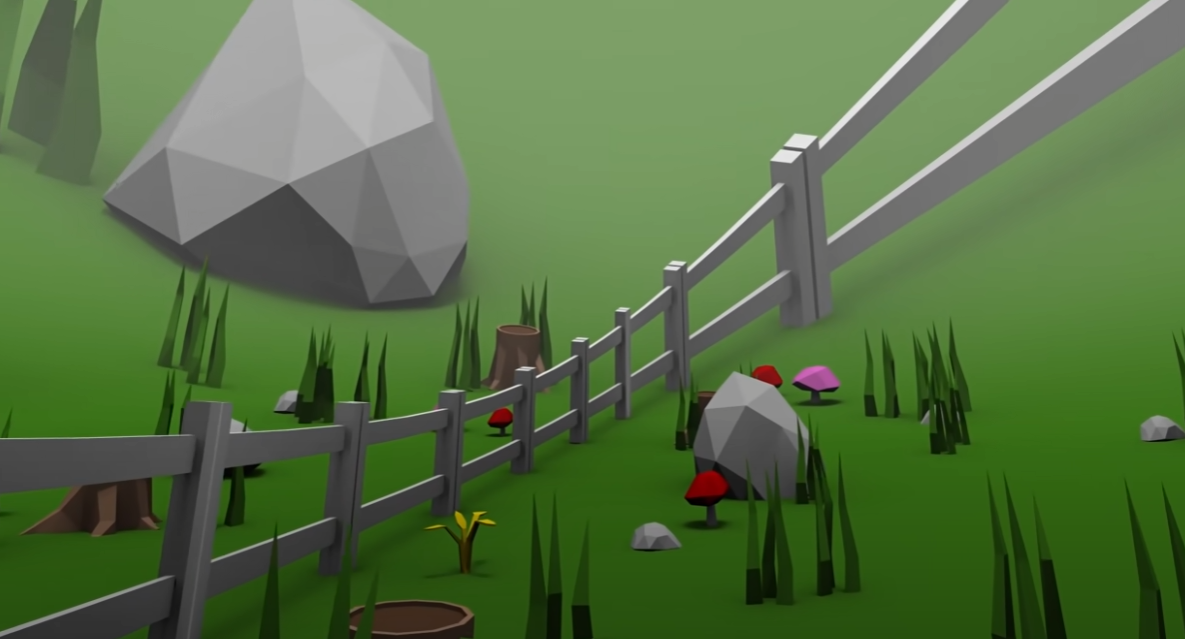
\includegraphics[width=\textwidth]{chapters/results/sections/non_euclidean/resources/hyperbolica-1.png}
        \caption[]%
        {{\small \textit{Hyperbolica \cite{Hyperbolica-Spherical}}}}
        \label{fig:spherical-space-games-hyperbolica}
    \end{subfigure}
    \caption[]
    {\small Spherical space}
    \label{fig:spherical-space-games}
\end{figure*}

The effect of characters bending increasingly as the player gets further from them is another example of an unusual visual effect in spherical space.
Furthermore, unlike in Euclidean geometry, objects further from the player do not always appear smaller, sometimes they can even appear larger.
This effect of "reversed perspective" can be seen in both games as shown in \autoref{fig:spherical-space-reversed-perspective}.
In \autoref{fig:spherical-space-reversed-perspective-hyper}, the car and the bot to the right of the car's hood are further from the camera than other objects in the scene.
\begin{figure*}[h]
    \centering
    \begin{subfigure}[b]{0.475\textwidth}
        \centering
        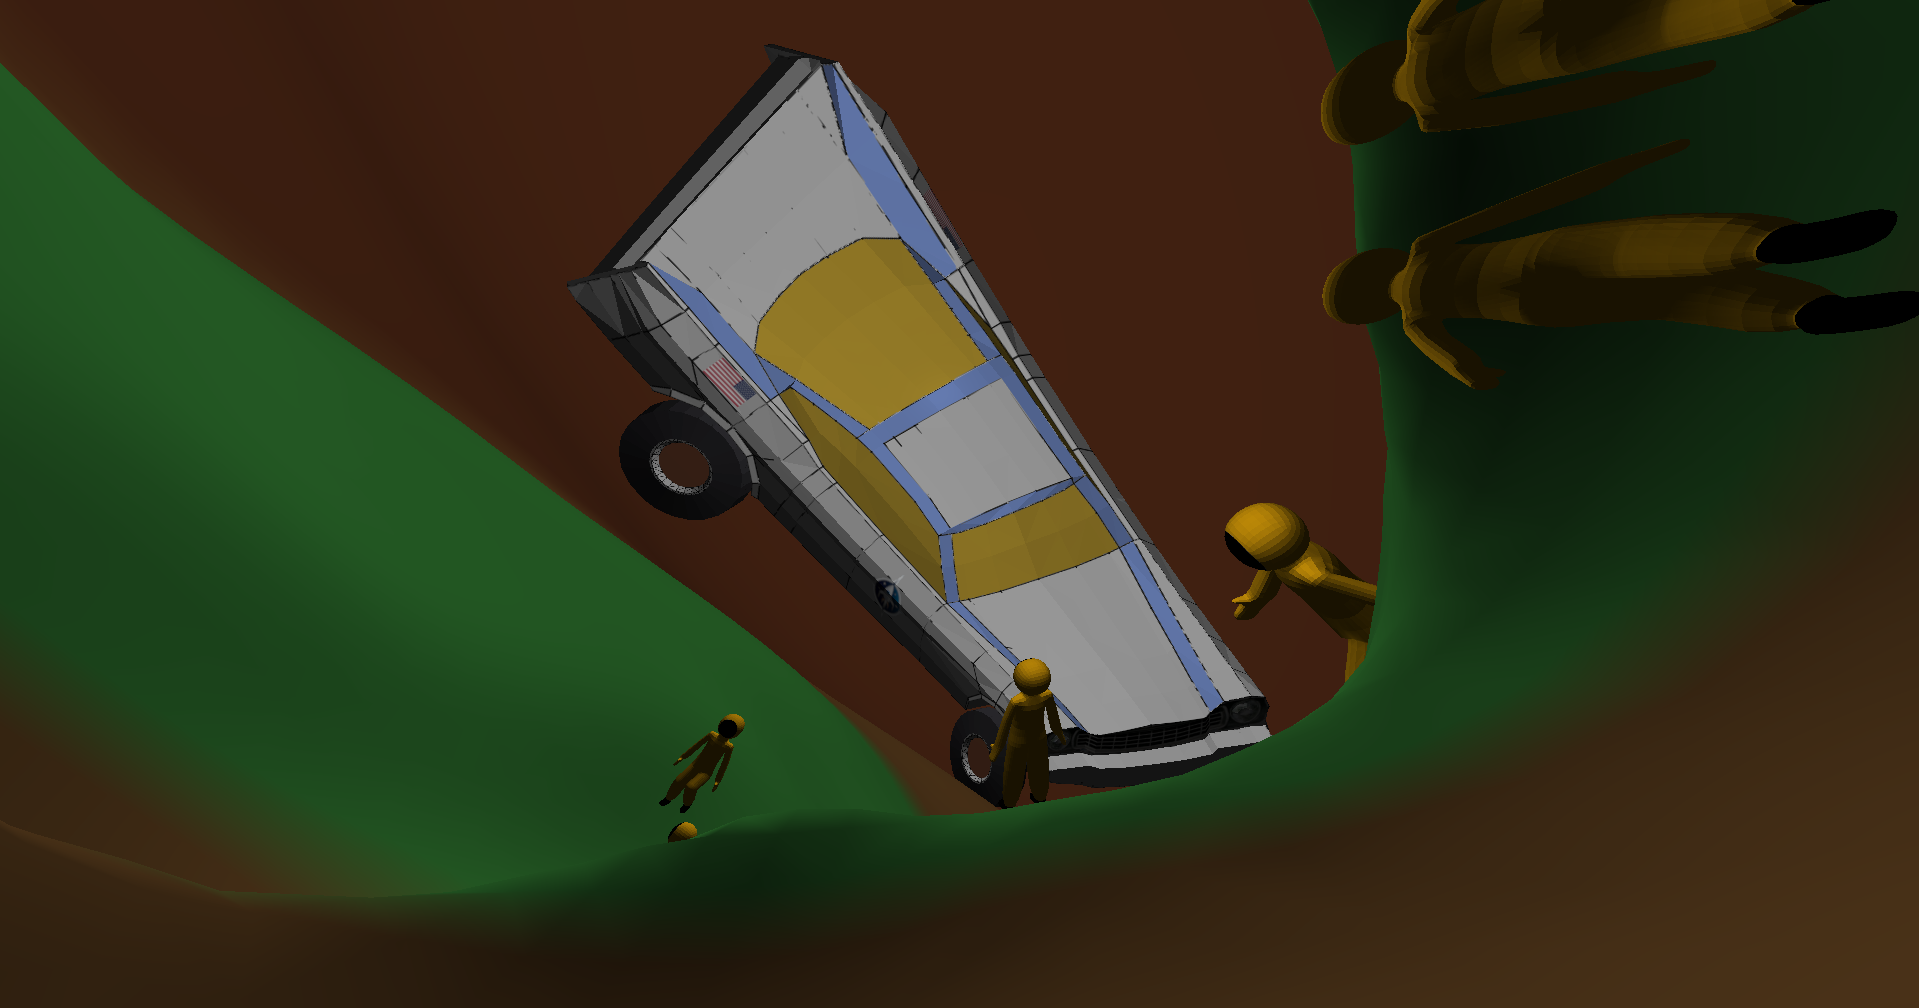
\includegraphics[width=\textwidth]{chapters/results/sections/non_euclidean/resources/spherical-car.png}
        \caption[]%
        {{\small \textit{Hyper}}}
        \label{fig:spherical-space-reversed-perspective-hyper}
    \end{subfigure}
    \hfill
    \begin{subfigure}[b]{0.5\textwidth}
        \centering
        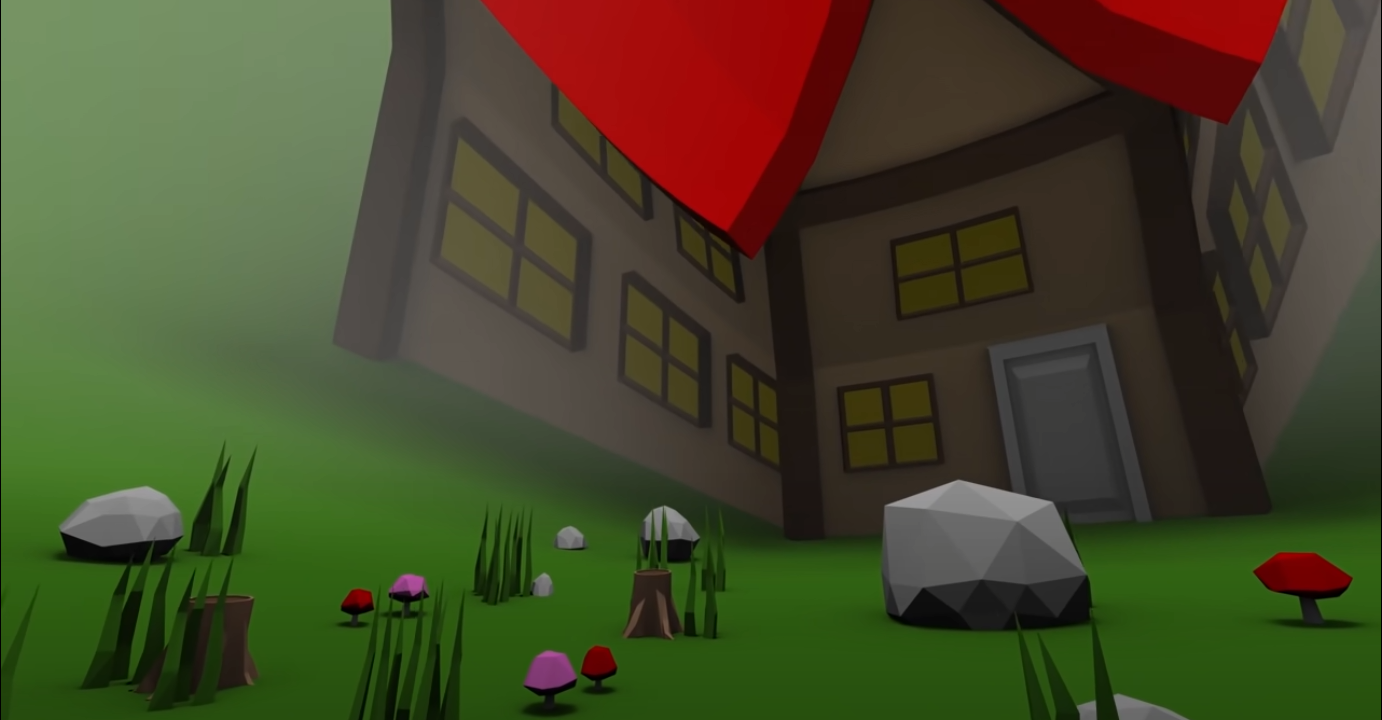
\includegraphics[width=\textwidth]{chapters/results/sections/non_euclidean/resources/hyperbolica-2.png}
        \caption[]%
        {{\small \textit{Hyperbolica}}}
        \label{fig:spherical-space-reversed-perspective-hyperbolica}
    \end{subfigure}
    \caption[]
    {\small Reversed perspective}
    \label{fig:spherical-space-reversed-perspective}
\end{figure*}
It's also important to note that bullets no longer fly in straight lines and that their trajectory is bent instead.
By playing the game it can be experienced that steering the car or moving the player's character appears unintuitive close to either of the spheres' boundaries.